\documentclass[12pt, letterpaper]{article}
\usepackage[english]{babel}
\usepackage{graphicx}
\usepackage{float}
\usepackage{hyperref}

\title{DAT510 - Assignment 1}
\author{Fr\o ydis J\o rgensen}

\begin{document}
\begin{titlepage}
\maketitle
\end{titlepage}


\begin{abstract}
For the first part of this assignment, I have decrypted a poly-alphabetic cipher without knowing the key. This was done by using factors between duplicated words and the chi-square statistic. I have looked into the execution time at different key lengths and a different cipher with the same key as the previous cipher trying to determine the differences. The second part of this assignment focuses on SDES and tripleSDES. There you will find the results to different test cases, where we found the ciphertext and plaintext bits by decrypting and encrypting knowing the key(s). Following there is an explanation of the filtering strategies.
\end{abstract}

\section*{Part 1}
\textbf{The plaintext message you managed to decipher} \\
\\
The plaintext message I got when I decrypted the cipher was:\\
\textit{
ANORIGINALMESSAGEISKNOWNASTHEPLAINTEXTWHILETHE\\CODEDMESSAGE
ISCALLEDTHECIPHERTEXTTHEPROCESSOF\\CONVERTINGFROMPLAINTEXT
TOCIPHERTEXTISKNOWNAS\\ENCIPHERINGORENCRYPTIONRESTORINGTHE
PLAINTEXTFROM\\THECIPHERTEXTISDECIPHERINGORDECRYPTIONTHEMANY
SCHEMES\\USEDFORENCRYPTIONCONSTITUTETHEAREAOFSTUDYKNOWNAS
CRYPTOGRAPHYSUCHASCHEMEISKNOWNASACRYPTOGRAPHIC\\SYSTEMORA
CIPHERTECHNIQUESUSEDFORDECIPHERINGAMESSAGE\\WITHOUTANY
KNOWLEDGEOFTHEENCIPHERINGDETAILSFALLINTO\\THEAREAOFCRYPTANALYSIS
CRYPTANALYSISISWHATTHELAY\\PERSONCALLSBREAKINGTHECODETHEAREASOF
CRYPTOGRAPHY\\ANDCRYPTANALYSISTOGETHERARECALLEDCRYPTOLOGY}\\
\\
\textbf{Describe the strategy you employed, show the details for each of the steps of that strategy, describe any programs you wrote, show sample output of these programs, and show how you transformed that output into your solution.} \\
\\
To solve the Poly-alphabetic Ciphers I started by determining what kind of cipher algorithm that is used.
The best-known polyalphabetic cipher is called The Vigenére cipher. It is mainly two steps to decrypt this cipher.
We have to identify the length of the key and then find the actual key. 

To find the length of the key I used a test based on taking the factors of the periods. I needed to find strings that repeated trough the ciphertext and chose to add strings of length 3 and longer. Therefore my outer for-loop starts at 3, as shown in Figure \ref{fig:findKeyLength}. The algorithm searches through the whole ciphertext and if a string with length longer than 3 occurs more than once, we add it to the list \textit{wordsFrequently}. This part of the algorithm did I found here \cite{SE}.
\\ \\
\begin{figure}[H]
  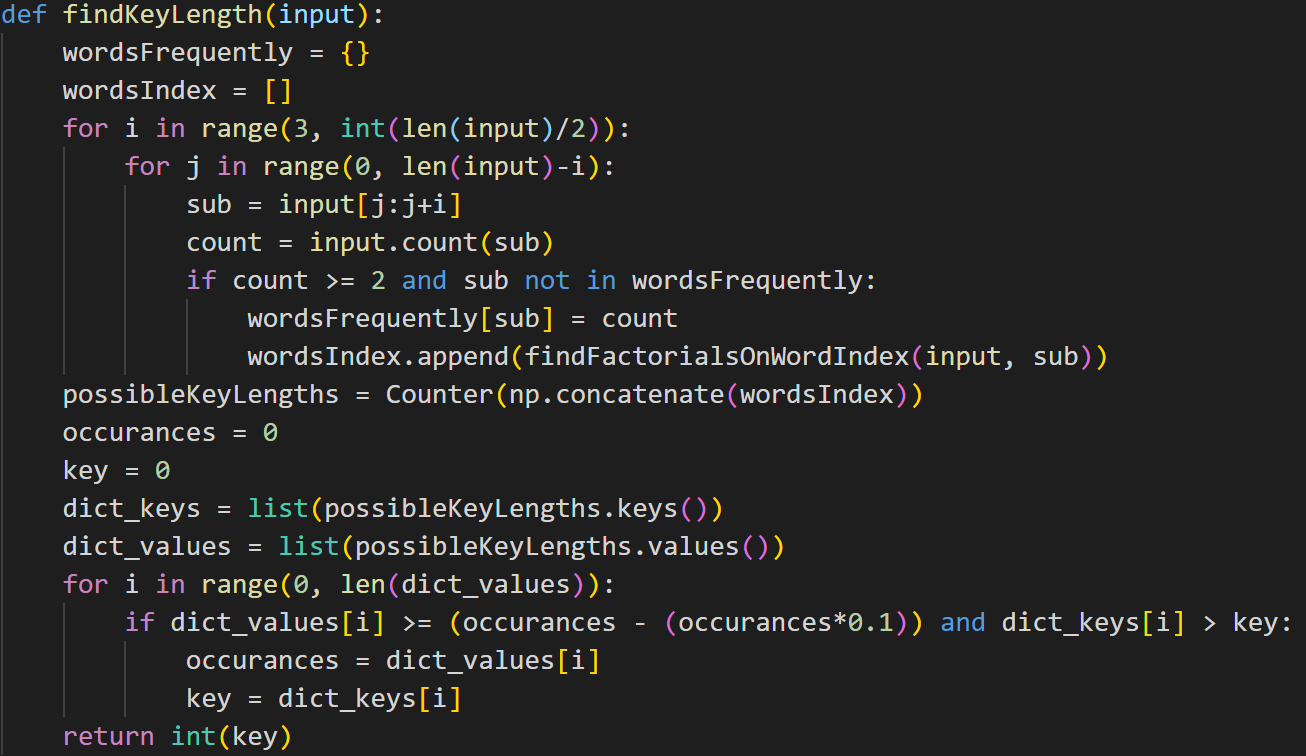
\includegraphics[width=\linewidth]{code_snippets/findKeyLength.PNG}
  \caption{the function to find key length}
  \label{fig:findKeyLength}
\end{figure}

To get the index I used the function \textit{findIndexOfDuplicates} that is highly inspired by one of the answers in this StackOverflow question, \cite{SO}. Figure \ref{fig:findIndexOfDuplicates} shows the function \textit{findIndexOfDuplicates} where the indexes of the substrings is added to a list and returned. \\ \\

\begin{figure}[H]
  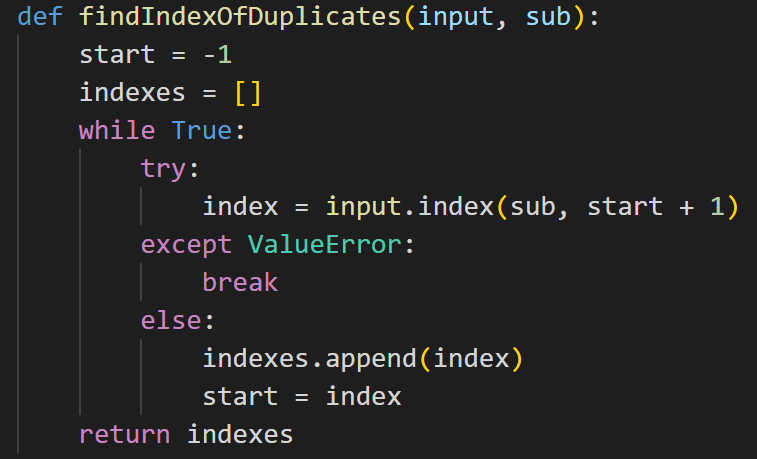
\includegraphics[width=\linewidth]{code_snippets/findIndexOfDuplicates.PNG}
  \caption{the function to find the indexes of duplicated strings}
  \label{fig:findIndexOfDuplicates}
\end{figure}

This method is used in the function \textit{findFactorialsOnWordIndex} as shown in Figure \ref{fig:findFactorialsOnWordIndex}. I then used the distance between the indexes of the repeated words and factorize it. I get the factors when the modulo of the index distance and \textbf{i} is zero. We got information that the key would be no larger than 10, therefore I only collected the factors in the range of 2 to 10.

\begin{figure}[H]
  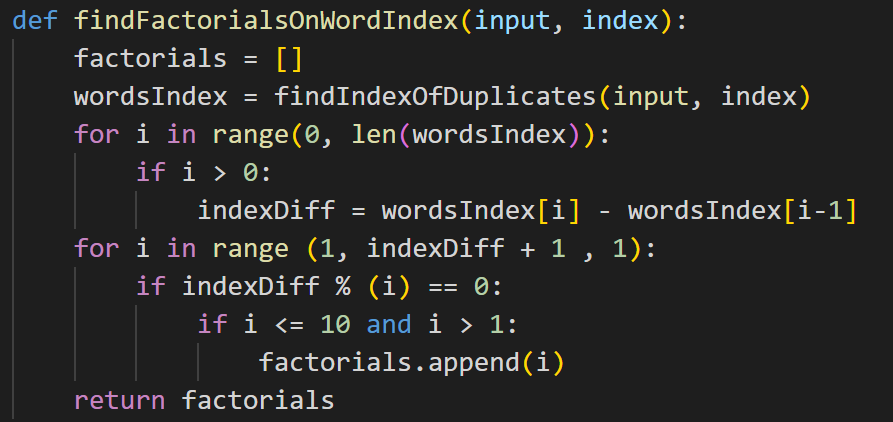
\includegraphics[width=\linewidth]{code_snippets/findFactorialsOnWordIndex.PNG}
  \caption{the function to find factorials}
  \label{fig:findFactorialsOnWordIndex}
\end{figure}

The next step in Figure \ref{fig:findKeyLength} to find the key length is to count the occurrence of the factors. The method I used to find the key length is based on using the highest factor that most often occurs. In this case, both 2, 4, and 8 occurred 105 times. The if-sentence at the end of Figure \ref{fig:findKeyLength} sets the key to be the highest factor that most often occurs, which in this case is 8.
\\ \\
Now that we know the length of the key we have to find the actual key. We know the period of the Vigenere cipher now is 8, which means that we have 8 caesar ciphers to break. I chose to use the Chi-squared statistic. The chi-squared statistic measures how similar two categorical probability distributions are. In this case, I wanted to compare the frequency distribution of the ciphertext characters and the frequency distribution of English.
\\ \\
As can see in the first for-loop in Figure \ref{fig:findKey}, I split my cipher in 8 strings, so I get a string witch consist of index [0,8,16,24 ...], [1,9,17, 25 ..], [2,10, 18, 26, ...] and so on. Then I count the occurrence of every letter in each of these 8 strings. To do that I use the function \textit{countLetters} as shown in Figure \ref{fig:countLetters}. When I have the letter occurrences I send the letter occurrences to perform the chi-square statistic and compare it to the English letter frequency.

\begin{figure}[H]
  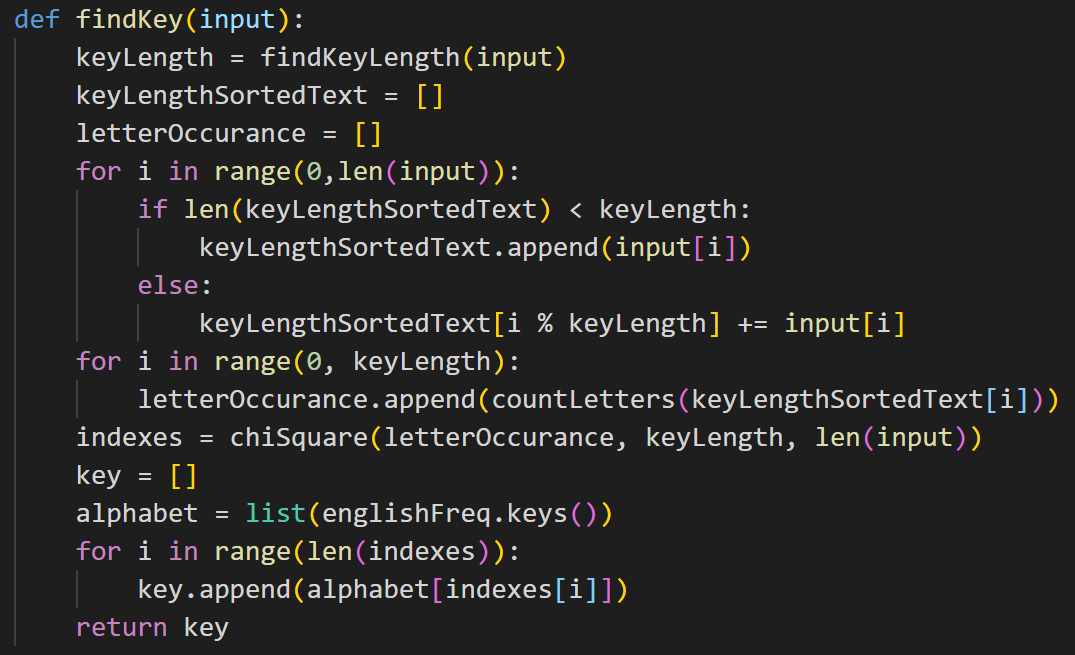
\includegraphics[width=\linewidth]{code_snippets/findKey.PNG}
  \caption{the function to find the key}
  \label{fig:findKey}
\end{figure}

\begin{figure}[H]
  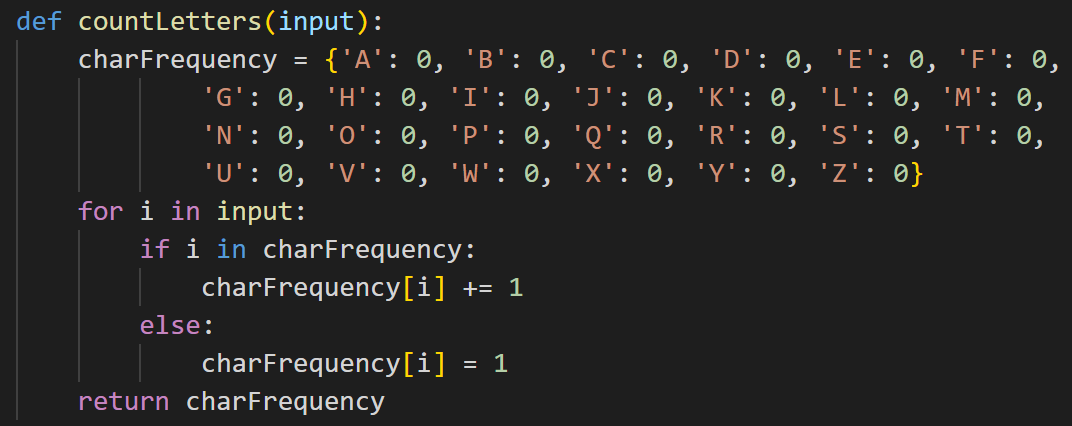
\includegraphics[width=\linewidth]{code_snippets/countLetters.PNG}
  \caption{the function count the occurance of letters}
  \label{fig:countLetters}
\end{figure}

The chi-square statistic is based on the formula: 
$$\sum_{i = Z}^{i = A} (Ci - Ei)^{2}/Ei $$
Where i is going through all of the letters in the English alphabet so that \textit{Ca} is the count of the letter the A, and \textit{Ea} is the expected count of the letter A. As shown in Figure \ref{fig:chiSquare} we loop through every letter inside a loop of every letter and we do once for each of the 8 strings we have gotten previously. The chi-square statistic says that the letter with the lowest sum in each of the strings is a part of our key \cite{chi}. In this example the \textit{chiSquare} function returns an array of \textbf{[1,3,11,0,4,10,2,24]}. This array tells us at which index the letters lays on. Since the index starts at zero, The first letter will be B. The key is, therefore, as we find in the last for-loop in Figure \ref{fig:findKey}, when we convert the indexes back to letters \textbf{BDLAEKCY}. \\ \\

\begin{figure}[H]
  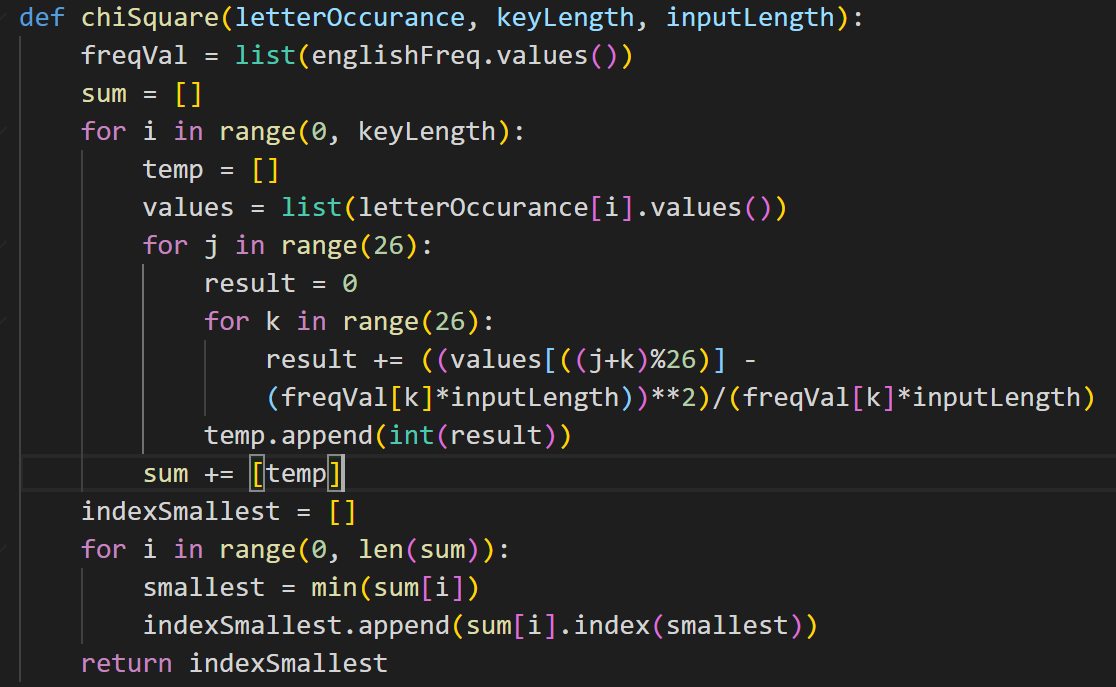
\includegraphics[width=\linewidth]{code_snippets/chiSquare.PNG}
  \caption{the function to find the smallest index}
  \label{fig:chiSquare}
\end{figure}

With the knowledge of what the key is, the only thing that is lest is to decrypt the cipher by using the key. A Vingere Cipher is decrypted by only using substitution, therefore it is an easy process of decrypting it when you know the key. As shown in Figure \ref{fig:vigenereDecrypt} I convert the key and the input into a list of Unicodes. Unicode is a superset of ASCII. I go through the cipherUnicode value by value and subtract it by the keyUnicode that belongs to the cipher's Unicode index. Then We take the modulo of the length of the English alphabet. This gives us values in the specter of 0 to 25. To convert it back to normal letters I add 65 to the Unicode value and cast it back to letters. After going through all of the letters we have the decrypted message in plaintext.

\begin{figure}[H]
  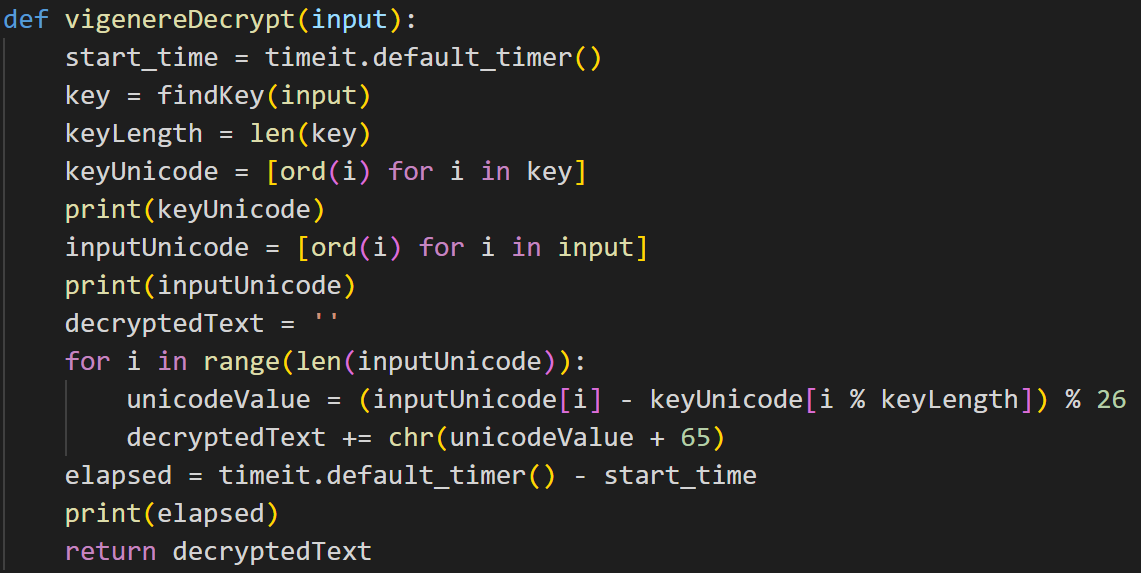
\includegraphics[width=\linewidth]{code_snippets/vigenereDecrypt.PNG}
  \caption{the main function to decrypt vigenere cipher}
  \label{fig:vigenereDecrypt}
\end{figure} 


When it comes to task 3, which had been encrypted by the same key as the previous ciphertext with an addition in the encryption process, it did not work to use the same tool as created for Task 1. This is probably because it's added substitution or permutation, which means it's not encrypted by the vigenere cipher. When I use the same key to decrypt the cipher I get the first 7 characters correct, but the rest of the text is gibberish.
\\ \\
\textbf{Describe the Execution time and impact of the key length on it.}
\\ \\
\begin{center}
\begin{tabular}{ |c|c| } 
 \hline
 Length of key & Execution time \\
 8 & 0.308 \\ 
 2 & 0.379 \\
 4 & 0.306 \\
 5 & 0.378 \\
 10 & 0.363 \\
 20 & 0.308 \\
 30 & 0.390 \\
 100 & 0.470 (wrong plaintext) \\
 \hline
\end{tabular}
\end{center}

According to my numbers, there is no significant difference in the execution time when the keys are at length between 2 and 30. The numbers are also most likely affected by the capacity of my computer is that exact moment which makes the numbers less valuable. My algorithm does not work very accurately when the key length is bigger than 30, so when I tried with a key length of 100 it gave me the wrong plaintext. As you can see the execution time did increase, but it is not much slower overall and the inaccuracy of my computer can misleading. Overall I think you need a really large key to make any significant difference in the execution time, and the capacity of the computer probably makes the biggest difference.
\newpage
\section*{Part 2}
\textbf{The result of test cases in Tasks 1 and 2}

\subsubsection*{Task 1 results}
\begin{center}
\begin{tabular}{ |c|c|c| } 
 \hline
 Raw key & Plaintext & Ciphertext \\
 0000000000 & 00000000 & 11110000 \\ 
 0000011111 & 11111111 & 11100001 \\ 
 0010011111 & 11111100 & 10011101 \\ 
 0010011111 & 10100101 & 10010000 \\ 
 1111111111 & 11111111 & 00001111 \\
 0000011111 & 00000000 & 01000011 \\
 1000101110 & 00111000 & 00011100 \\
 1000101110 & 00001100 & 11000010 \\
 \hline
\end{tabular}
\end{center}

\subsubsection*{Task 2 results}
\begin{center}
\begin{tabular}{ |c|c|c|c| } 
 \hline
 Raw key 1 & Raw key 2 & Plaintext & Ciphertext \\
1000101110 & 0110101110 & 11010111 & 10111001 \\
1000101110 & 0110101110 & 10101010 & 11100100 \\
1111111111 & 1111111111 & 00000000 & 11101011 \\
0000000000 & 0000000000 & 01010010 & 10000000 \\
1000101110 & 0110101110 & 11111101 & 11100110 \\
1011101111 & 0110101110 & 01001111 & 01010000 \\
1111111111 & 1111111111 & 10101010 & 00000100 \\
0000000000 & 0000000000 & 00000000 & 11110000\\
 \hline
\end{tabular} 
\end{center} 

\textbf{The bits making up the keys of the SDES and TripleDES in Task 3}
\\ \\
The key that cracks the SDES cipher is: \textbf{1111101010}. \\
The keys that cracks the tripleSDES cipher is: \\ Key 1: \textbf{1111101010} \\ Key 2: \textbf{0101011111}
\\ \\
\textbf{Describe the filtering strategy you used to know that the keys are correct.}
\\ \\
\textbf{SDES} \\ 
To decide if the key was correct while going through all possible 10 bits keys I created a regex that only allowed letters in the English alphabet. So if one of the $2^{10}$ possible keys gives a decrypted message consisting of only characters in the English alphabet it is a large posiblity that that we have the correct keys. I therefore makes an educated guess that the key giving a decrypted message of only characters is the correct anwer. This aproach worked and returned a text that made sense.
\\ \\
\textbf{TripleSDES} \\
I used the same strategy as for SDES. But tripleSDES needs two 10 bits keys. So with this method we have to do $2^{10}$ operations $2^{10}$ times. Because we have to go through every possible \textit{key 2} for every possible \textit{key 1}. This makes this algorithm much slower than SDES, and sometimes it uses up to 3 minutes to bruteforce TripleSDES.


\section*{Conclusion}
This assignment was a real challenge, but by doing some research on vigenere ciphers and following the recipe on SDES it was possible to decrypt the ciphers. If I should continue working on my programs I would like to make my vigenere cipher algorithm good enough to handle longer keys and still get the correct plaintext. When it comes to SDES and tripleSDES I think it's many ways to optimize the execution time so that tripleSDES don't use 3 minutes to decrypt one sentence. 

\newpage
\begin{thebibliography}{10} 
\bibitem{SE} StackExchange., \emph{Algorithm to find unknown patterns in a string},
\url{https://cs.stackexchange.com/questions/79182/im-looking-for-an-algorithm-to-find-unknown-patterns-in-a-string}.
\bibitem{SO} StackOverflow, . \emph{Index of duplicated items},
\url{https://stackoverflow.com/questions/5419204/index-of-duplicates-items-in-a-python-list}
\bibitem{chi} Practical cryptography, . \emph{Chi-squared Statistic},
\url{http://practicalcryptography.com/cryptanalysis/text-characterisation/chi-squared-statistic/#javascript-chi-squared-calculator}
\end{thebibliography}



\end{document}